\worksheet{Scoring Confidence}

\textbf{Scoring Like Alex Morgan}
See if you score a goal in a cap:
\begin{enumerate}
	\item Roll a die.
	\item If you roll a 1, 2, 3, or 4, you score; else you don't.	
	\item Repeat this ten times and keep track of your progress with the chart below.
\end{enumerate}
\begin{center}
		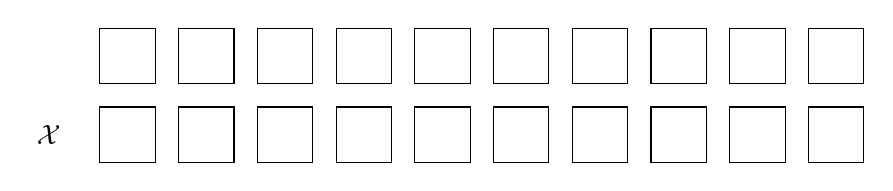
\begin{tikzpicture}
	\node at (0,1) {$\checkmark$};
	\node at (0,0) {$\mathcal{X}$};
		 \foreach \x in {1,...,10}{
		\foreach \y in {0,...,1}{
       \node [inner sep=10pt, draw] at  (\x,\y)  {};
       }
			}
	\end{tikzpicture}
\end{center}
\vfill
\textbf{Creating a Program}
\begin{itemize}
	\item For each game, pick a uniform random number between 0 and 1.
	\item If the number is less than 0.629, Morgan scores in the game. Else, she doesn't.
	\item Play 159 games, tally the number of games in which she scores, and compute the goals/cap rate.
	\item Repeat ten thousand times.
\end{itemize}

\begin{itemize}
	\item What simplifying assumptions are we making in our program?\vfill
	\item What would you change in the program if you were running a simulation for Mia Hamm? \vfill
\end{itemize}
